\documentclass[koma,a4paper]{article}
\usepackage[T1]{fontenc}
\usepackage[danish]{babel}
\usepackage{fixltx2e}
\usepackage{graphicx}
\usepackage{float}
\usepackage{amsmath}
\usepackage{amssymb}
\usepackage[hidelinks]{hyperref}
\usepackage{amsthm}
\usepackage{tikz}
\usepackage{todonotes}
\usepackage{booktabs}
\usepackage{subcaption}
\usepackage{color}
\usepackage{lmodern}
\graphicspath{{graphics/}}
\usetikzlibrary{trees}

\newcommand*\circled[1]{\tikz[baseline=(char.base)]{\node[shape=circle,draw,inner sep=2pt] (char) {#1};}} % circles around numbers

\title{AALG Self Study 2}
\author{Andreas Petersen\\
Mads E. Kalør\\
Søren B. Ranneries\\
Room 1.1.34}
\begin{document}
\maketitle

\pagebreak

\section{Exercise 1}

\subsection{Part a}
Suppose $S(a)$ is an optimal solution for the amount $a$. Then we show that the greedy choice (take the largest coin first) is optimal for the coins $\circled{25}, \circled{10}, \circled{5}, \circled{1}$.

Suppose $a \geq 25$ and $\circled{25} \notin S(a)$ then:

\begin{align*}
  25 \times \circled{1} &\Rightarrow 1 \times \circled{25}, \text{ is } 24 \text{ coins less}\\
  5 \times \circled{5} &\Rightarrow 1 \times \circled{25}, \text{ is } 4 \text{ coins less}\\
  2 \times \circled{1}, 1 \times \circled{5} &\Rightarrow 1 \times \circled{25}, \text{ is } 2 \text{ coins less}\\
  \dots
\end{align*}

Suppose $10 \leq a < 25$ and $\circled{10} \notin S(a)$ then:

\begin{align*}
  10 \times \circled{1} &\Rightarrow 1 \times \circled{10}, \text{ is } 9 \text{ coins less}\\
  2 \times \circled{5} &\Rightarrow 1 \times \circled{10}, \text{ is } 1 \text{ coins less}\\
  1 \times \circled{5}, 5 \times \circled{1} &\Rightarrow 1 \times \circled{10}, \text{ is } 5 \text{ coins less}
\end{align*}

Suppose $5 \leq a < 10$ and $\circled{5} \notin S(a)$ then:

\begin{align*}
  5 \times \circled{1} &\Rightarrow 1 \times \circled{5}, \text{ is } 4 \text{ coins less}
\end{align*}

\hfill\ensuremath{\blacksquare}

\subsection{Part b}
Suppose $a \geq c^k$ and $\circled{$c^k$} \notin S(a)$ then:

\begin{align*}
  c \times \circled{$c^{k-1}$} &\Rightarrow 1 \times \circled{$c^k$}, \text{ is } c - 1 \text{ coins less}\\
  c^2 \times \circled{$c^{k-2}$} &\Rightarrow 1 \times \circled{$c^k$}, \text{ is } c^2 - 1 \text{ coins less}\\
  c^3 \times \circled{$c^{k-3}$} &\Rightarrow 1 \times \circled{$c^k$}, \text{ is } c^3 - 1 \text{ coins less}\\
  \dots\\
  c^{k-1} \times \circled{$c^1$} &\Rightarrow 1 \times \circled{$c^k$}, \text{ is } c^{k-1} - 1 \text{ coins less}\\
  c^k \times \circled{$c^0$} &\Rightarrow 1 \times \circled{$c^k$}, \text{ is } c^k - 1 \text{ coins less}\\
\end{align*}

The proofs for the subproblems are similar. One just works one's way from $c^{k-1} \leq a < c^k$ to $c^1 \leq a < c^2$.

\hfill\ensuremath{\blacksquare}

\section{Exercise 2: Exam Sheet Exercise 1}
\subsection{Sub Exercise 1}
If the emp cannon is activated during the 2nd second, it will kill $\text{min}(10, f(2 - 0)) = 3$ robots. It does not matter if the cannon is fired during the third or the fourth second. If the cannon is activated during the third second, it will only have charged up enough to kill 1 robot. If it is fired during the fourth second only, it can kill 3 robots, but there is only 1 robot to kill. The optimal strategy is to activate it during the third and fourth second. It will then kill a total of 5 robots.

If the cannon is not activated during the 2nd second it will kill no robots during the second second. If the cannon is fired during the third second it will kill $\text{min}(10, f(3 - 0)) = 6$ robots. It can then be fired again the fourth second and kill 1 robot. It does not pay of to save the cannon for fourth second, as there is only one robot to kill then. The optimal strategy is then to fire the cannon at the third and fourth second, killing a total of 7 robots.

If the cannon is activated during the first second it will kill $\text{min}(1, f(1 - 0)) = 1$ robot. Then the optimal strategy is to fire the cannon during the third second, where it will kill $\text{min}(10, f(3 - 1)) = 3$ robots. It can then be fired again in the fourth second to kill 1 robot, resulting a total of 5 kills.

\subsection{Sub Exercise 2}
On the input shown in Table \ref{tab:shed_cannon_bad_input} the Schedule-Cannon will give the incorrect answer. It will fire during the 1, 4 and 5 second killing 7 robots. The optimal solution is to fire during the 3, 4, and 5 second killing a total of 8 robots.

\begin{table}[htp]%
  \centering
  \begin{tabular}{llllll}
    \toprule
    $i$ & \textbf{1} & \textbf{2} & \textbf{3} & \textbf{4} & \textbf{5} \\
    \midrule
    $x_i$  & 1 & 5 & 10 & 5 & 1 \\
    $f(i)$ & 1 & 3 & 6 & 9 & 12 \\
    \bottomrule
  \end{tabular}
\caption{Input to Schedule-Cannon}
\label{tab:shed_cannon_bad_input}
\end{table}

\subsection{Sub Exercise 3}
The recurrence for the problem, where $j$ is the number of seconds since the cannon was last fired and $\mathcal{X}$ is the sequence $x_1, x_2, \dots x_n$, can be seen in Equation \ref{eq:robot_cannon_recurrence}.

\begin{align}
  s(j, \mathcal{X}) = \begin{cases}
    \text{min}(x_1, f(j)) &\text{if } |\mathcal{X}| = 1 \\
    \text{max}\left(\begin{aligned}
      &s(1, \mathcal{X}.\text{remove}(x_1)) + \text{min}(x_1, f(j)),\\
      &s(j + 1, \mathcal{X}.\text{remove}(x_1))
    \end{aligned}\right) &\text{otherwise}
  \end{cases}
  \label{eq:robot_cannon_recurrence}
\end{align}

Figure \ref{fig:ex_2_table} shows the table that we need to fill out. The arrows inside the table represents the subproblems that the subproblem, from which the arrow originates, needs to know. The arrow on the far right indicates the order in which we need to fill the table --- starting top right and moving down and left.

Rows are seconds last fired from the cannon, and the columns is $x_i$.

\begin{figure}[htbp]
  \centering
  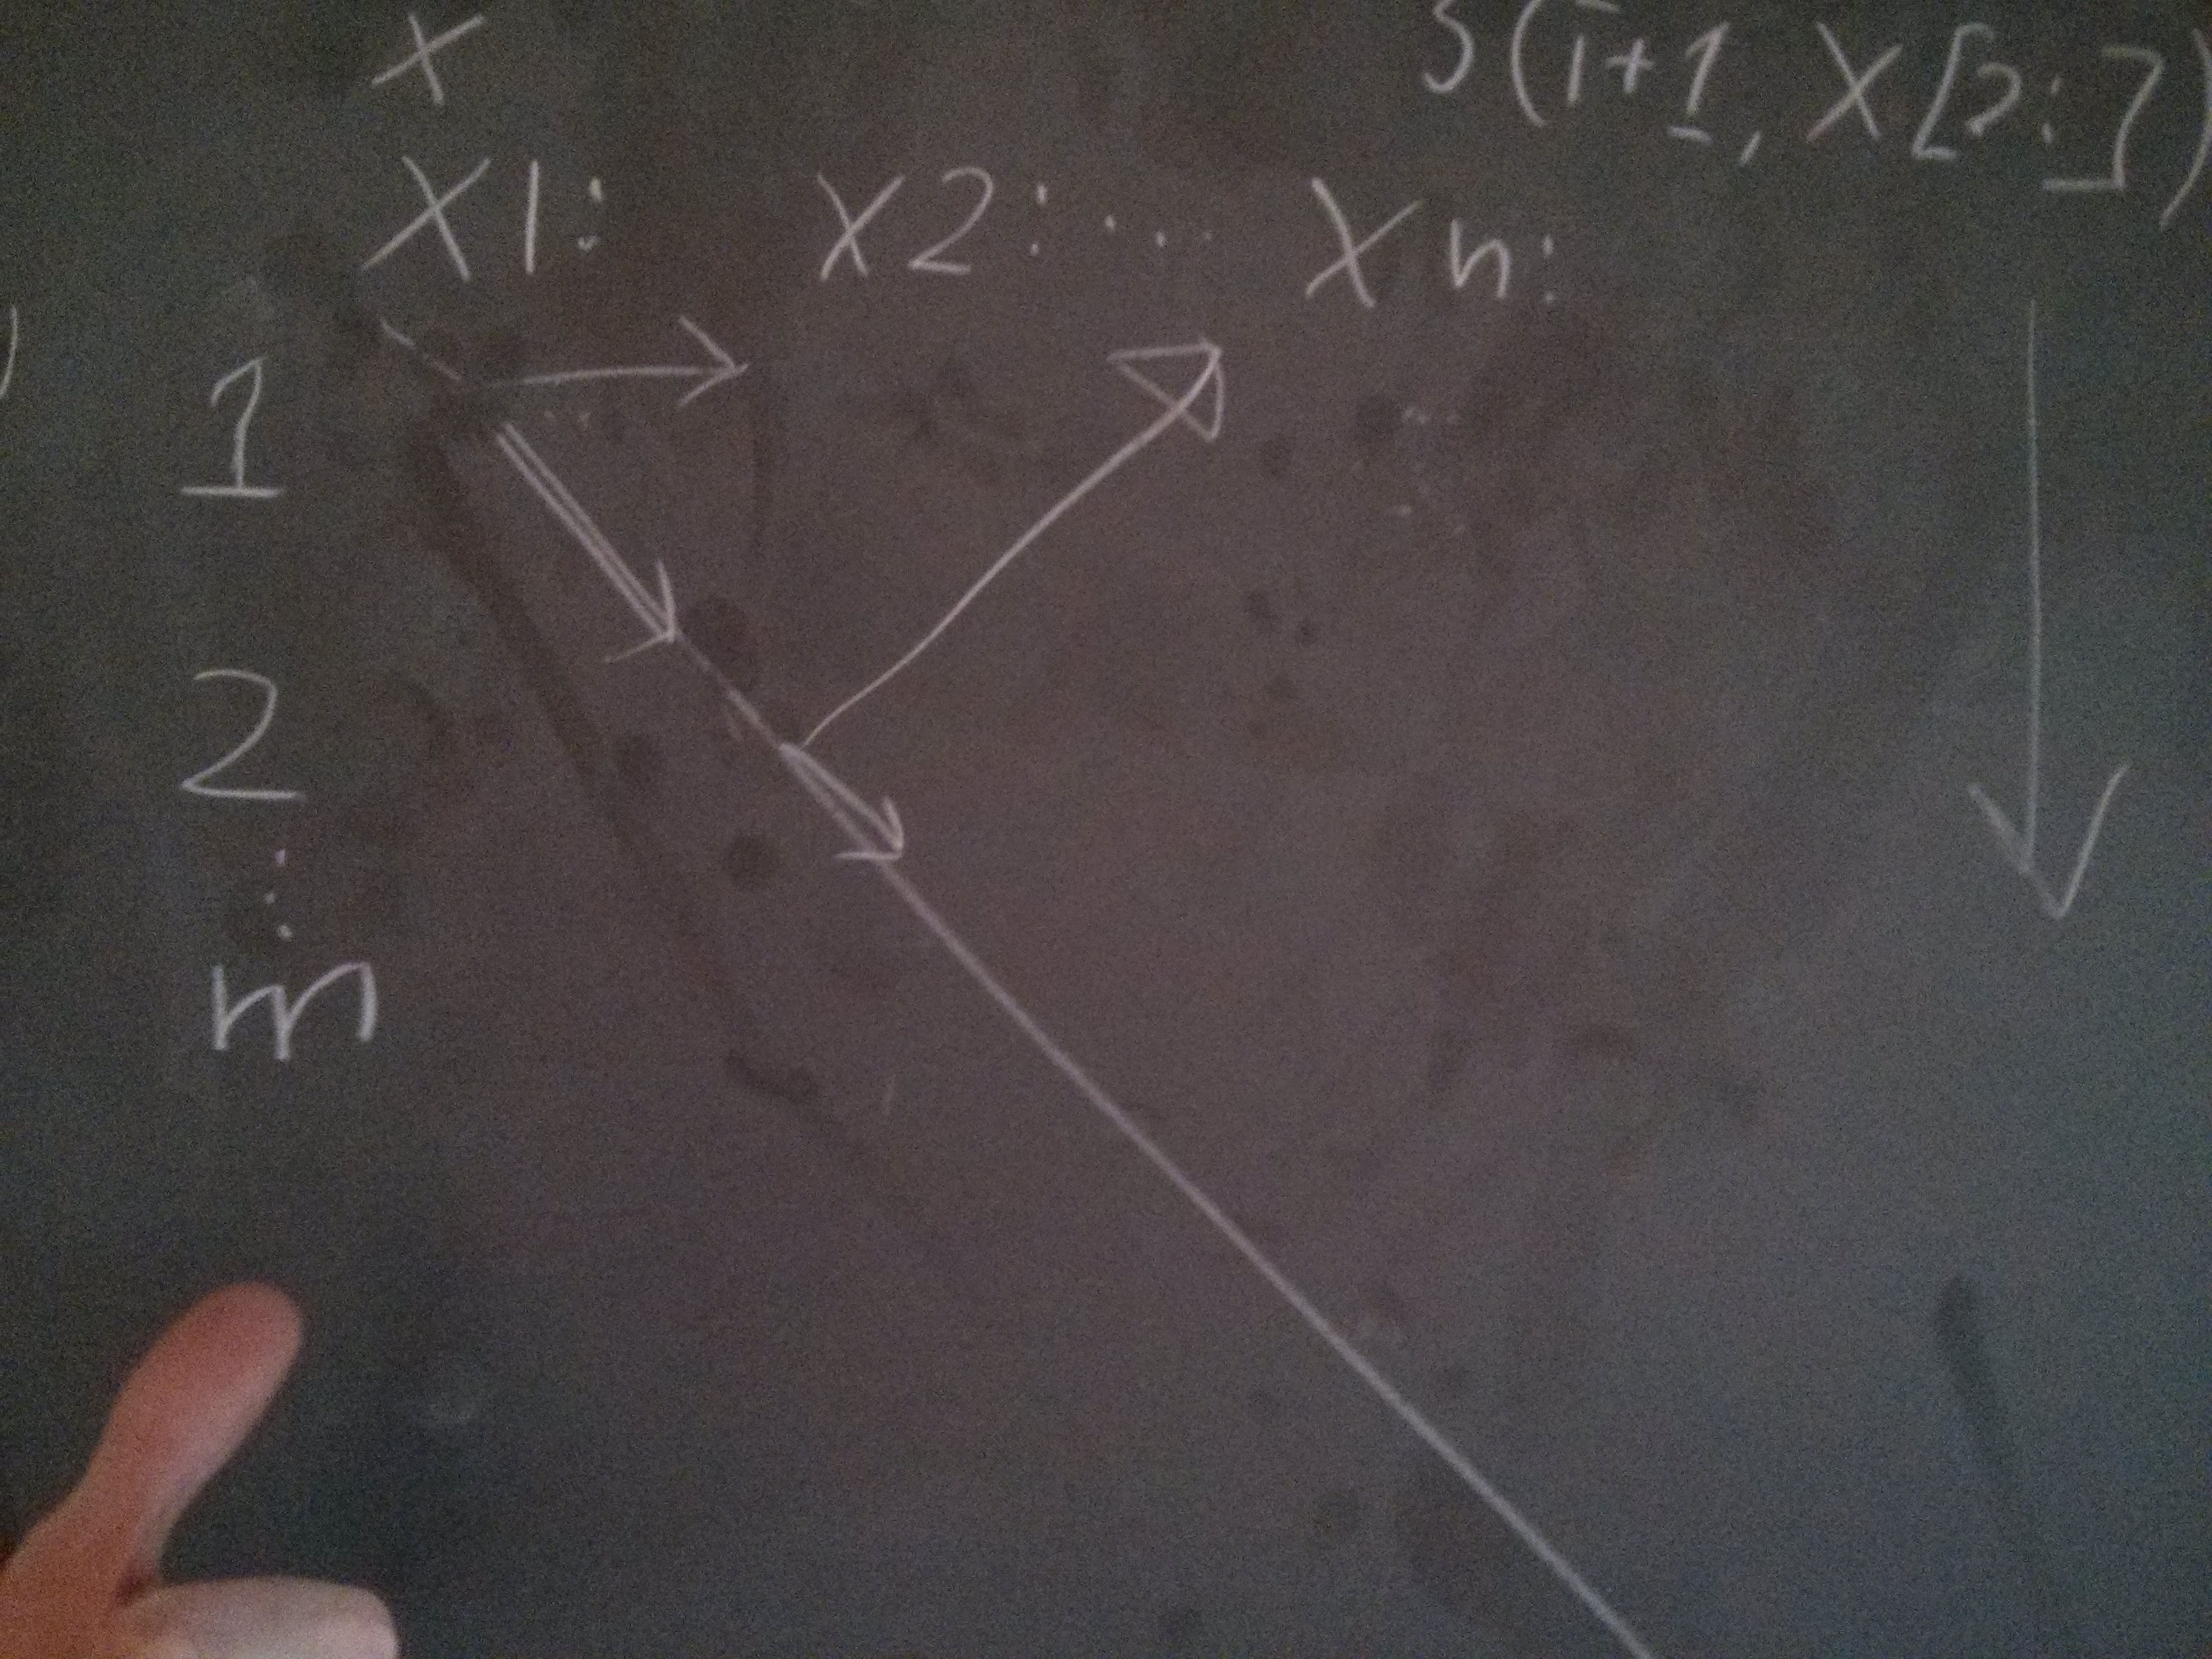
\includegraphics[width=1\textwidth]{ex_2_table}
  \caption{CSP fra STRIPS}\label{fig:ex_2_table}
\end{figure}

MostKills finds the most kills that can be achieved. MostKillsAug also stores the choices to make to kill most robots. They are bottom-up algorithms.

\begin{align*}
  &\text{MostKills}(\mathcal{X}, f)\\
  &~~~~\text{for } i \leftarrow n \text{ to } 1\\
  &~~~~~~~~\text{for } j \leftarrow 1 \text{ to } n\\
  &~~~~~~~~~~~~k \leftarrow \text{min}(x_i, f(j))\\
  &~~~~~~~~~~~~\text{if } i = n \text{ then}\\
  &~~~~~~~~~~~~~~~~m[i, j] = k\\
  &~~~~~~~~~~~~\text{else }\\
  &~~~~~~~~~~~~~~~~m[i, j] = \text{max}(m[i + 1, 1] + k, m[i + 1, j + 1])\\
  &~~~~\text{return } c[1, 1], s
\end{align*}

\begin{align*}
  &\text{MostKillsAug}(\mathcal{X}, f)\\
  &~~~~\text{for } i \leftarrow n \text{ to } 1\\
  &~~~~~~~~\text{for } j \leftarrow 1 \text{ to } n\\
  &~~~~~~~~~~~~k \leftarrow \text{min}(x_i, f(j))\\
  &~~~~~~~~~~~~\text{if } i = n \text{ then}\\
  &~~~~~~~~~~~~~~~~m[i, j] \leftarrow k\\
  &~~~~~~~~~~~~~~~~s[j] \leftarrow \top\\
  &~~~~~~~~~~~~\text{else }\\
  &~~~~~~~~~~~~~~~~m[i, j] \leftarrow \text{max}(m[i + 1, 1] + k, m[i + 1, j + 1])\\
  &~~~~~~~~~~~~~~~~\text{if } m[i + 1, 1] + k > m[i + 1, j + 1] \text{ then}\\
  &~~~~~~~~~~~~~~~~~~~~s[j] \leftarrow \top\\
  &~~~~~~~~~~~~~~~~\text{else}\\
  &~~~~~~~~~~~~~~~~~~~~s[j] \leftarrow \bot\\
  &~~~~\text{return } \langle c[1, 1], s \rangle
\end{align*}

Printing the solution can be done by enumerating $s$, where $s[i]$ indicates whether to shoot ($\top$) or not ($\bot$) at the $i$-th second. The running time of the algorithm is $\Theta(n^2)$ from the arithmetic series $\frac{n(n - 1)}{2}$.

\section{Exercise 3}
\subsection{Sub Exercise 1}
If the president is invited, then the highest level employees that can be invited is S-level employees. The maximum friendliness rating is $3 + 5 + 2 + 5 = 15$.

If the president is not invited, the highest level is V-level employees and the maximum friendliness rating is $6 + 5 + 2 + 3 = 16$.

\subsection{Sub Exercise 2}
The recurrence for the problem can be seen in Equation \ref{eq:company_party_recurrence}, where $T$ is the root of the tree. $T.f$ is the friendliness of $T$. $T.c$ is the children of $T$ and $T.\mathit{gc}$ is the grand children of $T$. While the tree structure does not have these functions, we abstract from the implementation details in the recurrence. The algorithm will, however, consider this.

\begin{align}
  c(T) = \begin{cases}
    T.f &\text{if } T.c = \text{null} \\
    \text{max}\left(\sum\limits_{t \in T.c} c(t), T.f + \sum\limits_{t \in T.\mathit{gc}} c(t)\right) &\text{otherwise}
  \end{cases}
  \label{eq:company_party_recurrence}
\end{align}

The algorithm that solves the problem is called MostFriendliness and is a memoized algorithm. $T.l$ is the left child of $T$. $T.r$ is the right sibling of $T$.

\begin{align*}
  &\text{MostFriendliness}(T, m)\\
  &~~~~\text{if } m[T] \neq \text{null then}\\
  &~~~~~~~~\text{return } m[T]\\
  &~~~~\text{if } T.l = \text{null then}\\
  &~~~~~~~~m[T] \leftarrow T.f\\
  &~~~~\text{else }\\
  &~~~~~~~~m[T] \leftarrow \text{max}\left(\text{sibsum}(T.l, m), \sum\limits_{t \in \text{sib}(T.l)} \text{sibsum}(t.l, m) + T.f \right)\\
  &~~~~\text{return } m[T]
\end{align*}

\begin{align*}
  &\text{sibsum}(T, m)\\
  &~~~~T' \leftarrow T\\
  &~~~~s \leftarrow \text{MostFriendliness}(T, m)\\
  &~~~~\text{while } T'.r \neq \text{null then}\\
  &~~~~~~~~s \leftarrow s + c(T'.r)\\
  &~~~~~~~~T' \leftarrow T'.r\\
  &~~~~\text{return } s
\end{align*}

\begin{align*}
  &\text{sib}(T)\\
  &~~~~T' \leftarrow T\\
  &~~~~l \leftarrow \text{new list}\\
  &~~~~\text{while } T'.r \neq \text{null then}\\
  &~~~~~~~~l.\text{add}(T'.r)\\
  &~~~~~~~~T' \leftarrow T'.r\\
  &~~~~\text{return } s
\end{align*}

The algorithm PrintGuestList prints the guest list.

\begin{align*}
  &\text{PrintGuestList}(T, m)\\
  &~~~~\text{if } \text{sibsum}(T.l, m) < \sum\limits_{t \in \text{sib}(T.l)}\text{sibsum}(t.l) + T.f \text{ then}\\
  &~~~~~~~~\text{print} T.\text{name}\\
  &~~~~~~~~\text{for } t \in \text{sib}(T.l)\\
  &~~~~~~~~~~~~\text{for } u \in \text{sib}(t.l)\\
  &~~~~~~~~~~~~~~~~\text{PrintGuestList}(u, m)\\
  &~~~~\text{else }\\
  &~~~~~~~~\text{for } t \in \text{sib}(T.l)\\
  &~~~~~~~~~~~~\text{PrintGuestList}(t, m)
\end{align*}

\subsection{Sub Exercise 3}
Each node in the tree (except the root and it's immediate children) are visited twice. The total running time of the algorithm is $\Theta(n)$, where $n$ is the number of nodes in the tree.

\end{document}